\chapter{Approccio proposto}
\label{chap:approccio}
\vspace{1cm}
Nel Capitolo \ref{chap:SOA} sono state descritte alcune soluzioni proposte 
relative al lavoro oggetto di questa tesi, in particolare algoritmi esatti ed
euristici di ottimizzazione atti a risolvere il problema di mapping e 
scheduling, congiuntamente o separatamente. Alla luce delle limitazioni dei 
lavori presentati è stato spiegato il motivo per cui si rende necessario questo 
lavoro di sviluppo di un baseline scheduler nell'ambito del progetto 
\ac{FASTER}.

In questo capitolo verrà descritto l'approccio utilizzato per risolvere il 
problema di scheduling dei task tenendo in considerazione le comunicazioni e 
riconfigurazioni introdotte.

Il capitolo è organizzato secondo la seguente struttura: nella Sezione 
\ref{sec:integrazioneToolchainFASTER} viene descritta l'integrazione 
dell'algoritmo di scheduling con il componente che gestisce il mapping dei task, 
con accenni alle interfacce esterne che collegano il componente 
con gli altri strumenti utilizzati nella toolchain di \acs{FASTER}; la Sezione 
\ref{sec:panoramicaMetodologia} descrive ad alto livello il funzionamento 
dell'algoritmo di scheduling, fornendo una panoramica delle fasi in cui questo 
si divide; la Sezione \ref{sec:euristicaSceltaTask} contiene una descrizione 
dettagliata della fase più delicata del procedimento di scheduling, la scelta 
del task migliore da considerare ad ogni passo di decisione; nella Sezione 
\ref{sec:elementiComunicazioneGestioneMemoria} vengono introdotti i modelli di 
comunicazione supportati dall'algoritmo proposto e una possibile allocazione 
statica della memoria per i task di computazione svolta contemporaneamente allo 
scheduling; infine, la Sezione \ref{sec:osservazioniConclusive} fornisce un 
riepilogo dei concetti importanti presentati in questo capitolo.


\section{Integrazione nella toolchain di \acs{FASTER}}
\label{sec:integrazioneToolchainFASTER}

Come descritto nel precedente capitolo, l'obiettivo del progetto europeo 
\ac{FASTER} è fornire un framework per la sintesi ad alto livello di 
applicazioni, scritte in linguaggio di programmazione C, su vari dispositivi 
riconfigurabili; la toolchain che permette di realizzare questa sintesi è 
composta da varie fasi eseguite in sequenza. Ogni fase deve essere il più 
possibile self-contained, ovvero deve poter essere invocata separatamente e non 
deve avere nozioni sul funzionamento interno delle altre fasi.

Condizione necessaria perchè ciò accada è la definizione di specifiche 
interfacce per ogni strumento che deve essere invocato. Ad esempio, la fase di 
mapping ha la propria interfaccia di input e di output; lo scheduler 
(incapsulato nell'algoritmo evolvibile di esplorazione delle soluzioni) ha 
anch'esso una interfaccia di input e una di output, contenenti tutte 
le strutture dati necessarie per l'elaborazione e per la memorizzazione delle 
informazioni calcolate dall'algoritmo, rispettivamente. 

%%% FIXME: color
\begin{figure}
 \begin{center}
  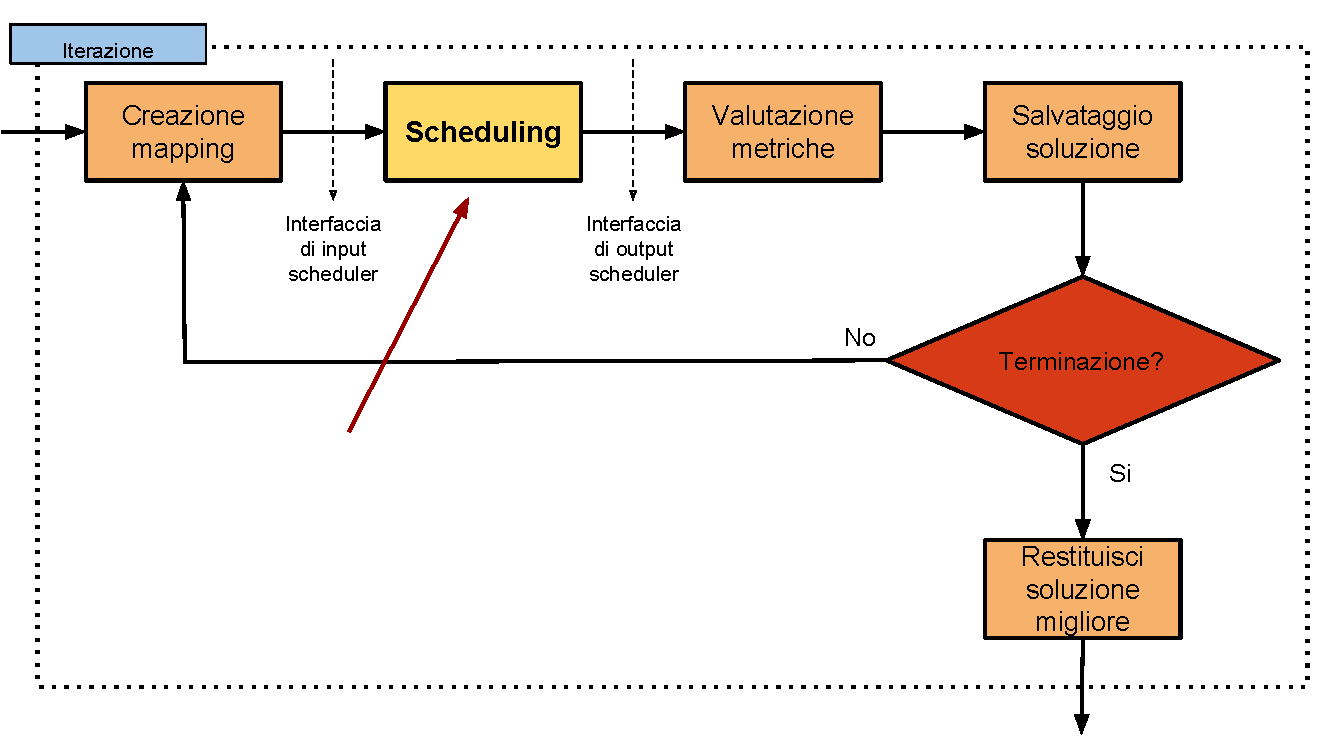
\includegraphics[width=0.9\textwidth]{capitoli/figure/cap3/MapperWorkflow.pdf}
  \caption{Flusso di lavoro dell'algoritmo di esplorazione.}
  \label{fig:mapperWorkflow}
 \end{center}
\end{figure}

A livello dell'algoritmo di esplorazione delle soluzioni, dunque, si avrà un 
flusso di lavoro come rappresentato nella Figura \ref{fig:mapperWorkflow}, in 
cui è messo in evidenza dove si colloca la fase di scheduling oggetto del 
lavoro, con le relative interfacce di input e output.

Anche la fase di mapping, che precede l'invocazione del tool che gestisce lo 
scheduling, è caratterizzata dalle proprie interfacce di input e output. Come 
si può vedere nella Figura \ref{fig:mapperWorkflow}, poichè la fase di 
scheduling è immediatamente successiva a quella di mapping, l'interfaccia di 
output del mapper e l'interfaccia di input dello scheduler avranno alcuni dati 
in comune.


\subsection{Interfaccia di input}

%%%%%%%%%%%% FIXME %%%%%%%%%%%%%
%%% overfull hbox %%%
\begin{figure}
 \begin{minipage}[b]{0.4\textwidth}
  \begin{center}
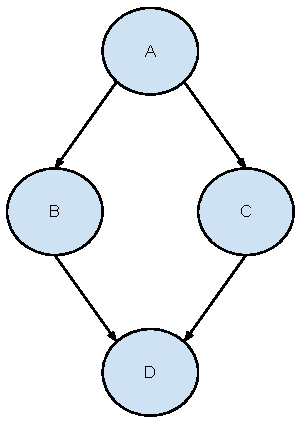
\includegraphics[width=\linewidth]{capitoli/figure/cap3/TaskGraphExample.pdf}
  \subcaption{Task graph}\label{fig:taskGraphExample2}
  \end{center}
 \end{minipage}
 \hfill
 \begin{minipage}[b]{0.4\textwidth}
  \begin{center}
   \begin{tabular}{| c | c | c |}
    \hline
    \textbf{Task} & \textbf{Component} & \textbf{Implementation}\\
    \hline
    A & p1 & impl\textunderscore0\\
    \hline
    B & p2 & impl\textunderscore1\\
    \hline
    C & p1 & impl\textunderscore2\\
    \hline
    D & p3 & impl\textunderscore3\\
    \hline
   \end{tabular}
   \subcaption{Lista dei mapping}\label{tab:listaMapping}
  \end{center}
 \end{minipage}
 \caption{Esempio di task graph e di lista dei mapping.}
 \label{fig:taskGraphAndMapping}
\end{figure}


L'interfaccia di input per la fase di scheduling contiene tutti i dati 
necessari all'esecuzione dello scheduler, alcuni definiti prima 
dell'invocazione del tool, altri creati o modificati durante le differenti fasi 
dell'esecuzione. In particolare, i dati definiti prima dell'invocazione sono:
\begin{itemize}
 \item dati provenienti dal file XML di specifica del progetto correntemente in 
elaborazione dalla toolchain, relativi alla descrizione dell'architettura, del 
task graph, delle implementazioni e dei vari elementi 
di computazione, di 
comunicazione e di memoria presenti;
 \item dati provenienti dall'output della fase di mapping.
\end{itemize}
Questi ultimi sono organizzati come una lista di triple \emph{$<$processing 
task, processing element, implementazione$>$} calcolata dal mapper, che 
specifica per ogni task:
\begin{enumerate}
 \item l'elemento di computazione che dovrà eseguire il task, può essere un 
core hardware su scheda oppure un soft core (processore);
 \item l'implementazione da utilizzare per l'esecuzione del task, si può 
dividere in implementazione software o hardware a seconda che il task debba 
essere eseguito su scheda o su un processore.
\end{enumerate}
Nella Figura \ref{fig:taskGraphAndMapping} sono rappresentati un esempio di 
task graph e di output della fase di mapping basato su quel task graph.

Le informazioni provenienti dal mapper vengono quindi utilizzate per 
determinare se alcune aree dovranno essere riconfigurate durante l'esecuzione 
dell'applicazione oppure no, oltre a dare informazioni sull'occupazione dei 
vari componenti del dispositivo.


\subsection{Interfaccia di output}

Il compito dello scheduler è assegnare delle stime di tempo di inizio e di fine 
esecuzione ad ogni task in modo che le precedenze tra i task imposte dal task 
graph vengano rispettate, e che nessun altro vincolo sia violato: ad esempio, 
task che devono essere eseguiti sullo stesso componente non possono avere tempi 
di esecuzione sovrapposti. Tutte queste informazioni sulle stime calcolate 
dallo scheduler vengono memorizzate nell'interfaccia di output, che è composta 
da:
\begin{itemize}
 \item una rappresentazione in forma di \emph{diagramma di Gantt}, che delinea 
per ogni componente quando questo è occupato nell'esecuzione di un task;
 \item per ogni task, una lista delle informazioni riguardanti lo scheduling, 
ad esempio il tempo d'esecuzione stimato, il componente su cui deve essere 
eseguito, l'implementazione che ne caratterizza l'esecuzione e le stime di 
inizio e fine esecuzione che gli sono state assegnate.
\end{itemize}

Nella prossima sezione verrà spiegato in dettaglio il flusso di 
esecuzione dell'algoritmo di scheduling e come le interfacce vengono 
utilizzate durante l'elaborazione.


\section{Panoramica della metodologia}
\label{sec:panoramicaMetodologia}

In questa sezione viene descritto il funzionamento dell'algoritmo proposto e le 
fasi in cui esso si articola, con una spiegazione dettagliata della struttura 
di ogni fase e del flusso di lavoro completo dell'algoritmo.

Come accennato nella sezione precedente, l'interfaccia di input è 
caratterizzata da dati ``statici'', presenti prima dell'invocazione dello 
scheduler e da dati ``dinamici'', che subiscono modifiche oppure vengono creati 
durante l'esecuzione del tool. L'interfaccia di output è invece costruita 
incrementalmente, aggiungendo e modificando dati man mano che la computazione 
prosegue.


\begin{figure}[ht]
 \begin{center}
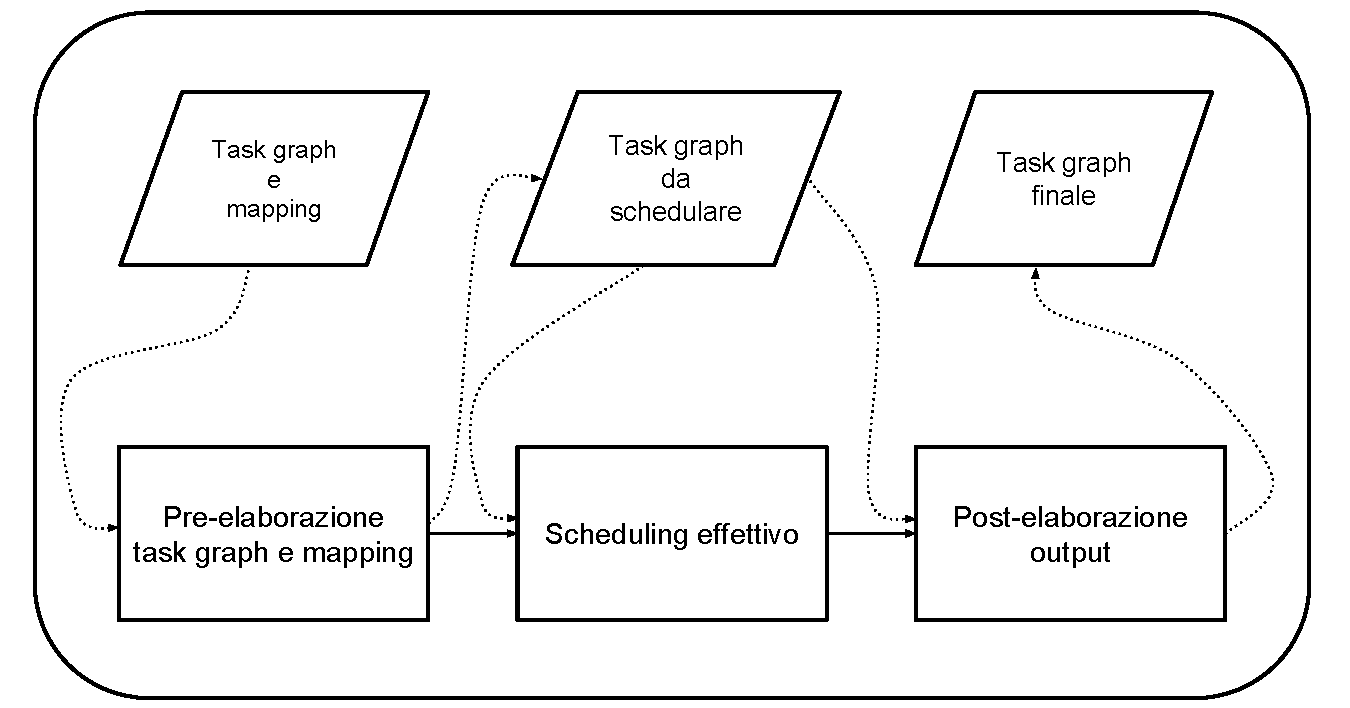
\includegraphics[width=0.9\textwidth]
{capitoli/figure/cap3/SchedulerWorkflow.pdf}
  \caption{Flusso di lavoro dell'algoritmo di scheduling.}
  \label{fig:schedulerWorkflow}
 \end{center}
\end{figure}


La prima fase dell'algoritmo ha il compito di 
effettuare una elaborazione preliminare dei dati statici, che permetterà di 
ottenere una formulazione più specifica e dettagliata del problema; questa 
prima fase è chiamata \emph{fase di preprocessing}. La seconda fase è 
costituita dallo \emph{scheduling effettivo} dei task, utilizzando le 
informazioni calcolate in precedenza nella pre-elaborazione. La terza e ultima 
fase, pur non essendo strettamente legata all'assegnazione delle stime dei tempi 
e dell'ordine di esecuzione dei task, è fondamentale per permettere l'effettiva 
esecuzione dell'applicazione sul dispositivo riconfigurabile; consiste in una 
parziale rielaborazione dell'output prodotto dalla fase di scheduling ed è 
chiamata \emph{fase di postprocessing}.

Le tre fasi sono rappresentate nella Figura \ref{fig:schedulerWorkflow}, che 
illustra il flusso di lavoro dello scheduler, con i relativi dati di input per 
ogni fase. Nelle prossime sezioni, ogni fase verrà analizzata nel dettaglio.


\subsection{Fase di preprocessing}
La fase di preprocessing è la prima ad essere eseguita dopo l'invocazione del 
tool di scheduling da parte dell'algoritmo di esplorazione. Ha come obiettivo 
principale l'identificazione delle comunicazioni e delle riconfigurazioni che 
devono essere prese in considerazione per la corretta esecuzione 
dell'applicazione sul dispositivo. Un obiettivo secondario è il calcolo di 
informazioni aggiuntive che verranno poi utilizzate nella fase di scheduling 
per quanto concerne la scelta del task migliore (vedi Sezione 
\ref{sec:euristicaSceltaTask}).

Per ottenere questi obiettivi, la fase di preprocessing si divide in tre 
sotto-fasi eseguite nel seguente ordine:
\begin{enumerate}
 \item aggiunta delle comunicazioni: nuovi task, detti \emph{task di 
comunicazione} vengono aggiunti al task graph originale, a rappresentare le 
comunicazioni che si verificano tra i task di computazione;
 \item aggiunta delle riconfigurazioni: può non essere richiesto e dipende 
dagli assegnamenti stabiliti dal mapping, consiste nell'introduzione di nuovi 
task, detti \emph{task di riconfigurazione}, dove necessario;
 \item computazione delle informazioni sul percorso critico.
\end{enumerate}

\subsubsection{Aggiunta delle comunicazioni}
L'inserimento dei task di comunicazione viene fatto solamente in base 
all'analisi del task graph dell'applicazione, in quanto indipendente dal 
mapping: dato che ogni arco in tale grafo rappresenta una relazione 
produttore-consumatore tra due task\footnote{Ovvero, denominati $i$ e $j$ i due 
task, un arco $(i,j)$ indica che l'output della computazione del task $i$ viene 
utilizzato come input per la computazione del task $j$.}, ogni arco viene 
trattato come una comunicazione.

Dati due task di computazione $i$, $j$ e un 
arco $(i,j)$ nel task graph, vi sono due tipi di task di comunicazione, che si 
differenziano per come operano il trasferimento dei dati:
\begin{itemize}
 \item task di comunicazione di tipo \emph{WRITE}, che \emph{scrivono} 
l'output del task $i$ in una memoria;
 \item task di comunicazione di tipo \emph{READ}, che \emph{leggono} dei dati 
da una memoria e li trasferiscono come input per il task $j$. 
\end{itemize}
Stanti queste premesse, ogni arco nel task graph implica l'inserimento di 
entrambi i tipi di task di comunicazione. L'arco originale viene rimosso e 
sostituito con nuovi archi che collegano i task di computazione con i task di 
comunicazione appena inseriti, rispettando i criteri precedentemente stabiliti.


\begin{figure}
 \begin{minipage}[b]{0.4\textwidth}
  \begin{center}
   $\vcenter{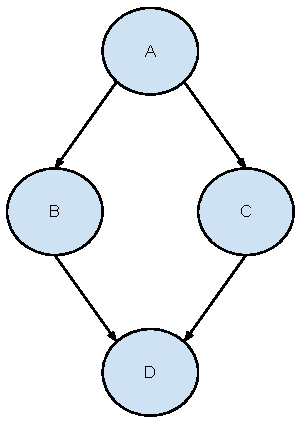
\includegraphics[width=\linewidth]
{capitoli/figure/cap3/TaskGraphExample.pdf}}$
  \end{center}
 \end{minipage}
 \hfill
 \begin{minipage}[b]{0.4\textwidth}
 \begin{center}
    $\vcenter{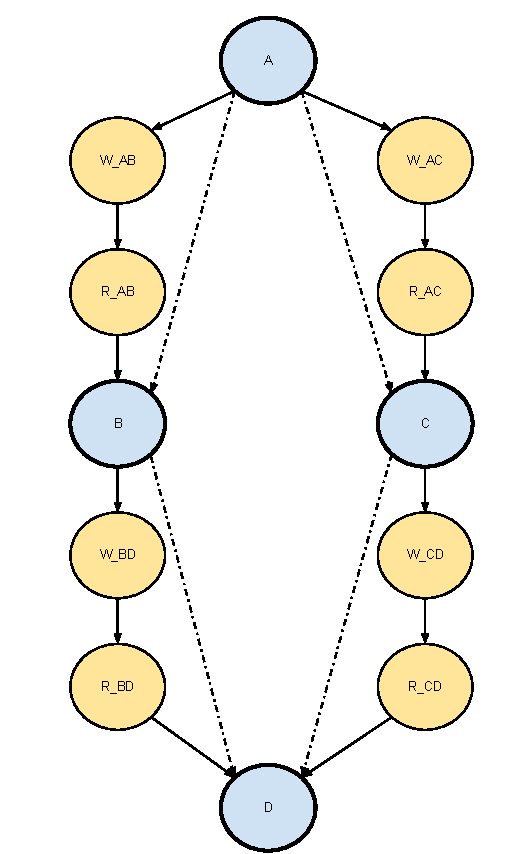
\includegraphics[width=\linewidth]
{capitoli/figure/cap3/TaskGraphCommunicationExample.pdf}}$
 \end{center}
 \end{minipage}
 \caption{Modifica del task graph in seguito all'aggiunta delle 
comunicazioni.}
 \label{fig:taskGraphCommunicationExample}
\end{figure}


Si veda la Figura \ref{fig:taskGraphCommunicationExample}
per un esempio di come viene modificato il task graph della Figura 
\ref{fig:taskGraphExample2} in seguito all'aggiunta dei task di 
comunicazione\footnote{Gli archi del grafo originale sono stati 
tratteggiati per evidenziare come la struttura generale non sia cambiata ma 
siano stati soltanto introdotti nuovi nodi e archi nel grafo.}.

Dopo l'inserimento dei task di comunicazione, viene eseguito l'inserimento dei 
task di riconfigurazione, qualora il particolare mapping utilizzato lo 
richieda. Nel caso, si procede come descritto nel prossimo paragrafo.


\subsubsection{Aggiunta delle riconfigurazioni}
\label{sec:aggiuntaRiconfigurazioni}
L'inserimento dei task di riconfigurazione avviene in seguito all'analisi della 
lista dei mapping fornita dal mapper ed è necessario nel caso in cui gli 
assegnamenti stabiliti dal mapper verifichino le seguenti condizioni:
\begin{enumerate}
 \item due task di comunicazione sono mappati sullo stesso componente 
(processing element);
 \item le implementazioni dei due task sono diverse e di tipo hardware, ovvero 
i due task devono essere eseguiti su logica riconfigurabile: questa condizione 
implica che il modulo hardware non sia riutilizzabile da parte del secondo task.
\end{enumerate}
Se queste condizioni sussistono per una qualsiasi coppia di task, allora 
un nuovo task di riconfigurazione deve essere aggiunto al grafo. Nella Tabella 
\ref{tab:esempioRiconfigurazione} è illustrato un esempio di quando si 
verificano le precedenti condizioni ed è necessario introdurre un nuovo task di 
riconfigurazione.

\begin{table}
\begin{center}
\begin{tabular}{| c | c | c |}
 \hline
    \textbf{Task} & \textbf{Component} & \textbf{Implementation}\\
    \hline
    A & \textcolor{red}{p1} & \textcolor{blue}{impl\textunderscore0}\\
    \hline
    B & p2 & impl\textunderscore1\\
    \hline
    C & \textcolor{red}{p1} & \textcolor{blue}{impl\textunderscore2}\\
    \hline
    D & p3 & impl\textunderscore3\\
    \hline
\end{tabular}
\caption{Esempio di riconfigurazione necessaria.}
\label{tab:esempioRiconfigurazione}
\end{center}
\end{table}


L'inserimento avviene seguendo un preciso criterio per l'introduzione delle 
dipendenze: non si può semplicemente inserire il nuovo task tra i due task di 
computazione e collegarlo a questi con dei nuovi archi, è necessario tenere 
conto delle comunicazioni appena introdotte. Ad esempio, dati due task di 
computazione $i$ e $j$ anche non adiacenti, non è possibile eseguire la 
riconfigurazione prima che l'output del task $i$ sia stato salvato in memoria 
perchè i dati sarebbero sovrascritti e non più disponibili; allo stesso tempo 
e per il medesimo motivo, non è possibile eseguirla dopo che i dati siano stati 
trasferiti come input per il task $j$. Questi vincoli determinano i seguenti
criteri di assegnazione delle precedenze:
\begin{itemize}
 \item nuovi archi sono introdotti da tutti i task di comunicazione di tipo 
\emph{WRITE} uscenti dal task $i$ al task di riconfigurazione;
 \item nuovi archi sono introdotti dal task di riconfigurazione a tutti i task 
di comunicazione di tipo \emph{READ} entranti nel task $j$.
\end{itemize}


\begin{figure}
 \begin{minipage}[b]{0.4\textwidth}
$\vcenter{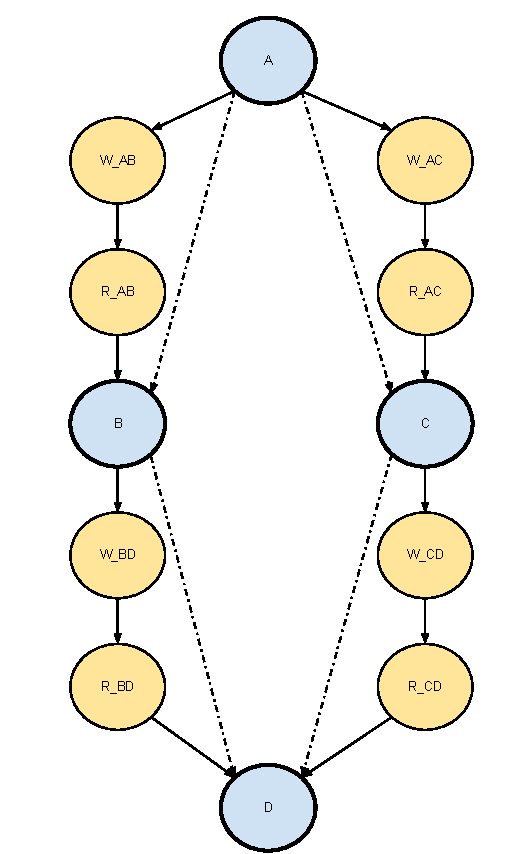
\includegraphics[width=\linewidth]
{capitoli/figure/cap3/TaskGraphCommunicationExample.pdf}}$
 \end{minipage}
 \hfill
 \begin{minipage}[b]{0.4\textwidth}
$\vcenter{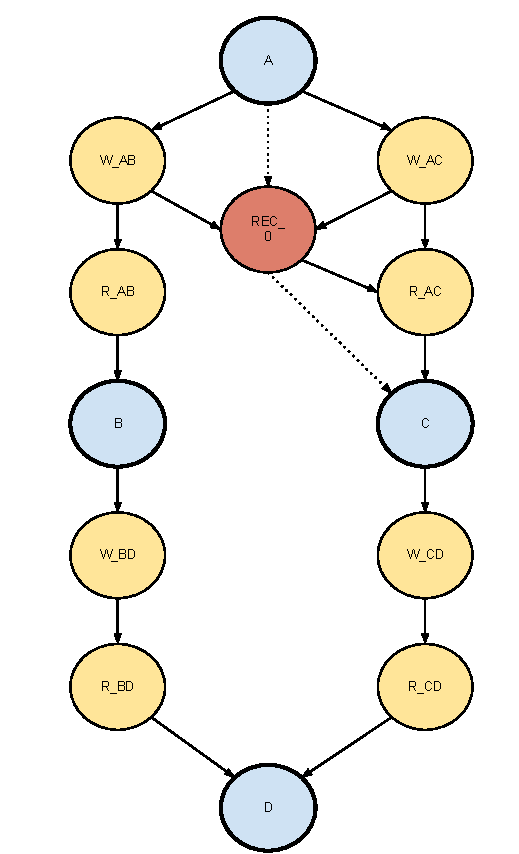
\includegraphics[width=\linewidth]
{capitoli/figure/cap3/TaskGraphCommRecExample.pdf}}$
 \end{minipage}
 \caption{Modifica del task graph in seguito all'aggiunta delle 
riconfigurazioni.}
 \label{fig:taskGraphCommRecExample}
\end{figure}


Nella Figura \ref{fig:taskGraphCommRecExample} è rappresentata l'evoluzione del 
task graph successiva all'introduzione dei task di riconfigurazione, sulla 
base dei mapping riportati nella Figura \ref{tab:listaMapping} e nella
Tabella \ref{tab:esempioRiconfigurazione}. Si può vedere il nuovo task di 
riconfigurazione introdotto, di colore rosso; gli archi entranti e uscenti dal 
nuovo task impongono le precedenze sopra elencate.

Una considerazione 
aggiuntiva riguarda gli archi tratteggiati che, nel grafo sulla destra, 
collegano i due task di computazione con il task di riconfigurazione: questi 
archi vengono inseriti in ogni caso durante il preprocessing, per esplicitare 
che deve verificarsi una riconfigurazione tra l'esecuzione del task $A$ e 
l'esecuzione del task $C$. La loro introduzione non influenza tuttavia il 
funzionamento dello scheduler. Le precedenze aggiuntive introdotte dal cammino 
$A \rightarrow REC\_0 \rightarrow C$ sono infatti dominate dai cammini già 
esistenti $A \rightarrow W\_AC \rightarrow REC\_0 \rightarrow R\_AC \rightarrow 
C$ e $A \rightarrow W\_AB \rightarrow REC\_0 \rightarrow R\_AC \rightarrow C$, 
quindi la presenza di tali archi non introduce nessun ritardo e non comporta 
svantaggi rispetto alla loro assenza.

Dopo l'aggiunta dei task di riconfigurazione, l'ultimo passo della fase di 
preprocessing consiste nel calcolo delle informazioni sul percorso critico del 
task graph.


\subsubsection{Calcolo delle informazioni sul percorso critico}
Le informazioni calcolate durante questa fase vengono utilizzate per stabilire 
quali task sono sul percorso critico\footnote{In inglese \emph{critical path}, 
avendo un grafo che simboleggia un progetto composto da attività (nodi) con 
precedenze (archi), rappresenta un cammino dal nodo iniziale al nodo finale del 
grafo costituito da attività che non possono essere ritardate senza allungare 
il tempo di esecuzione del progetto.}; verranno poi utilizzate nella fase di 
scheduling vero e proprio per l'assegnazione della priorità ai task

Tali informazioni consistono in tre dati, calcolati per ogni task del grafo 
preprocessato:
\begin{itemize}
 \item istante al più presto \emph{(asap)},
 \item istante al più tardi \emph{(alap)},
 \item scarto \emph{(slack)}: differenza tra istante al più tardi e istante al 
più presto.
\end{itemize}
I task con scarto pari a $0$ fanno parte del percorso critico.

Il calcolo delle tre informazioni sopra elencate viene effettuato tramite un 
semplice algoritmo comunemente utilizzato in ricerca operativa: il \ac{CPM}.
Vengono quindi aggiunti due \emph{nodi dummy}: sorgente, collegato ai nodi del 
grafo senza predecessori e destinazione, collegato ai nodi senza successori.
Il grafo viene poi ordinato topologicamente\footnote{Si noti che il task graph 
è aciclico quindi l'ordinamento topologico è sempre possibile.}, e l'algoritmo 
\ac{CPM} viene eseguito. Lo pseudocodice dell'algoritmo di ordinamento 
topologico è illustrato nell'Algoritmo \ref{alg:CPM}, dove $\delta^-(i)$ e 
$\delta^+(i)$ rappresentano il taglio entrante e il taglio uscente del nodo 
$i$, rispettivamente.

\IncMargin{1em}
\begin{algorithm}
 \SetKwInOut{Input}{input}\SetKwInOut{Output}{output}
 \SetKwArray{Asap}{asap}\SetKwArray{Alap}{alap}
 \SetKw{KwDownTo}{downto}
 
 \Input{Un grafo $G=(N,A)$, con $n = \vert N \vert$ e $d_i,\; \forall i = 
1,\dots,n$ durata del task $i$}
 \Output{$asap[i]$ e $alap[i],\; \forall i = 1,\dots, n$}
 \BlankLine
 \Asap{1} $\leftarrow 0$\;
 \For{$i = 2$ \KwTo $n$}{
 \Asap{i} $\leftarrow max\{$\Asap{p}$+ d_p\;:\;(p,i) \in \delta^-(i)\}$\;
 }
 \Alap{n} $\leftarrow$ \Asap{n}\;
 \For{$i=n-1$ \KwDownTo $1$}{
 \Alap{i} $\leftarrow min\{$\Alap{t}$- d_i\;:\;(i,t) \in \delta^+(i)\}$\;
 }
 \caption{Algoritmo CPM}
\label{alg:CPM}
\end{algorithm}
\DecMargin{1em}

Il calcolo delle informazioni sul percorso critico conclude la fase di 
preprocessing. Al termine di questa fase, il task graph presente 
nell'interfaccia di input dello scheduler viene sostituito con il grafo 
arricchito di comunicazioni e riconfigurazioni; le informazioni sul percorso 
critico appena calcolate sono aggiunte all'interfaccia, per essere utilizzate 
dalla fase successiva.


\subsection{Fase di scheduling}
\label{subsec:faseScheduling}
La fase di scheduling effettivo gestisce l'assegnazione di tempi di inizio e 
fine dell'esecuzione di ogni task, sia esso di computazione, comunicazione o 
riconfigurazione. In particolare, a condizione che le stime sulla durata dei 
task siano il più precise possibile, la fase di scheduling assegna un ordine di 
esecuzione dei task che rispetti tutte le precedenze imposte dal task graph e 
che cerchi di minimizzare il tempo di esecuzione \emph{stimato}.

\IncMargin{1em}
\begin{algorithm}
 \SetKwInOut{Input}{input}\SetKwInOut{Output}{output}
 \SetKwData{UnscheduledSet}{unscheduledSet}
 \SetKwData{SchedulerOutput}{schedulerOutput }
 \SetKwData{SchedulerInput}{schedulerInput}
 \SetKwData{BestTask}{bestTask}
 \SetKwData{ReadyTaskSet}{readyTaskSet}
 \SetKwData{TimeInfo}{timeInfo}
 
 \Input{the input interface of the scheduler}
 \Output{the output interface of the scheduler}
 \BlankLine
 \SchedulerOutput $\leftarrow \emptyset$\;
 \UnscheduledSet $\leftarrow$ \SchedulerInput.getTaskSet()\;
 \While{\UnscheduledSet is not empty}{
 \ReadyTaskSet $\leftarrow$ tasks with precedences satisfied\;
 \BestTask $\leftarrow$ best task to be scheduled among the ready tasks\;
 \TimeInfo $\leftarrow$ compute start/end time estimations for the best task\;
 \SchedulerOutput $\leftarrow$ \SchedulerOutput $\cup$ \TimeInfo\;
 \ReadyTaskSet $\leftarrow$ \ReadyTaskSet $\setminus$ \BestTask\;
 \UnscheduledSet $\leftarrow$ \UnscheduledSet $\setminus$ \BestTask\;
 }
 \Return{\SchedulerOutput}
\caption{Algoritmo per la fase di scheduling}
\label{alg:faseScheduling}
\end{algorithm}
\DecMargin{1em}

Come si può vedere nell'Algoritmo \ref{alg:faseScheduling}, la fase di 
scheduling è costituita principalmente da un ciclo ripetuto finchè vi sono 
task che non sono ancora stati schedulati. A ogni ripetizione del ciclo viene 
prima aggiornato l'insieme dei task che sono ``pronti'' per l'assegnazione dei 
tempi, ossia i task le cui precedenze sono state tutte già considerate. Tra 
questi, tramite un'opportuna euristica di scelta (vedi Sezione 
\ref{sec:euristicaSceltaTask}) viene eletto il miglior task da considerare al 
passo corrente; a questo vengono poi assegnate le stime dei tempi, 
successivamente inserite nell'interfaccia di output dello scheduler e nel 
diagramma di Gantt dei componenti occupati.

I dati di output dello scheduler vengono poi restituiti all'algoritmo di 
esplorazione che ha invocato il tool, e possono essere usati per avere una 
stima del tempo totale di esecuzione dell'applicazione.


\subsection{Fase di postprocessing}
Il postprocessing consiste in una rielaborazione dei dati di output dello 
scheduler, effettuata separatamente in quanto i dati prodotti in output da 
questa fase devono essere utilizzati solamente dal runtime manager per gestire 
l'esecuzione dell'applicazione.

\paragraph{Ruolo del runtime manager}
Poichè lo scheduler assegna degli istanti di inizio e fine dei task basati 
puramente su delle \emph{stime}, non vi è alcuna garanzia che tali istanti 
vengano rispettati nel corso di una reale esecuzione dell'applicazione sulla 
piattaforma riconfigurabile. Ciò vale soprattutto per i task la cui
durata di esecuzione è fortemente dipendente dalla quantità di dati da 
scambiare, da possibili conflitti sul BUS o sul canale di comunicazione 
utilizzato che rendono necessario serializzare le esecuzioni, nel caso di 
task di comunicazione, oppure dalla dimensione dell'area da configurare e 
dalle caratteristiche dell'architettura sottostante, nel caso di task di 
riconfigurazione.

Di fronte a questi errori nelle stime, non si può ritenere accurato il piano di 
esecuzione formulato dallo scheduler sotto forma di diagramma di Gantt; è 
necessario dunque che un componente si faccia carico dell'esecuzione dei vari 
task, lanciandone di nuovi quando i predecessori sono terminati: tale 
componente è il \emph{runtime manager}. Il ruolo del runtime manager è quello 
di coordinare le esecuzioni di tutti i task, rispettando le precedenze imposte 
dal grafo e l'ordine stabilito dallo scheduler.

\begin{figure}
 \begin{minipage}[b]{0.45\textwidth}
  $\vcenter{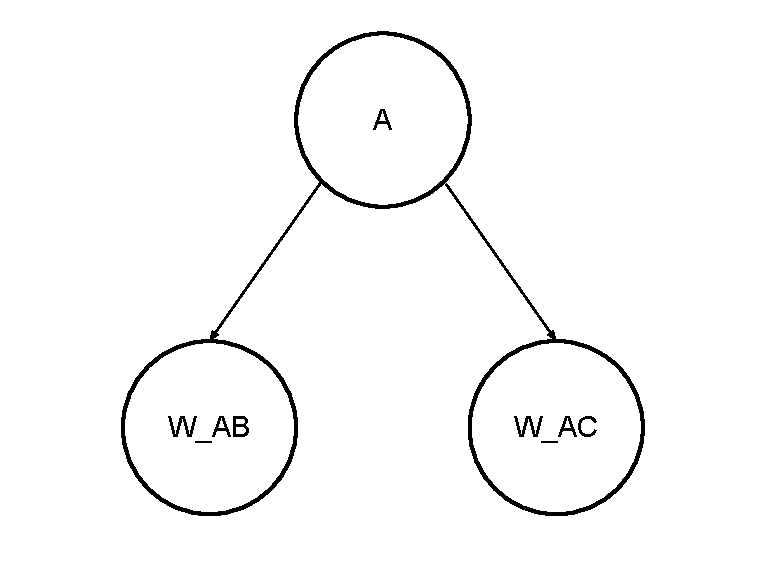
\includegraphics[width=\linewidth]
  {capitoli/figure/cap3/SchedulingConflict.pdf}}$
  \subcaption{Prima della risoluzione}
  \label{fig:schedulingConflictA}
 \end{minipage}
 \hfill
 \begin{minipage}[b]{0.45\textwidth}
  $\vcenter{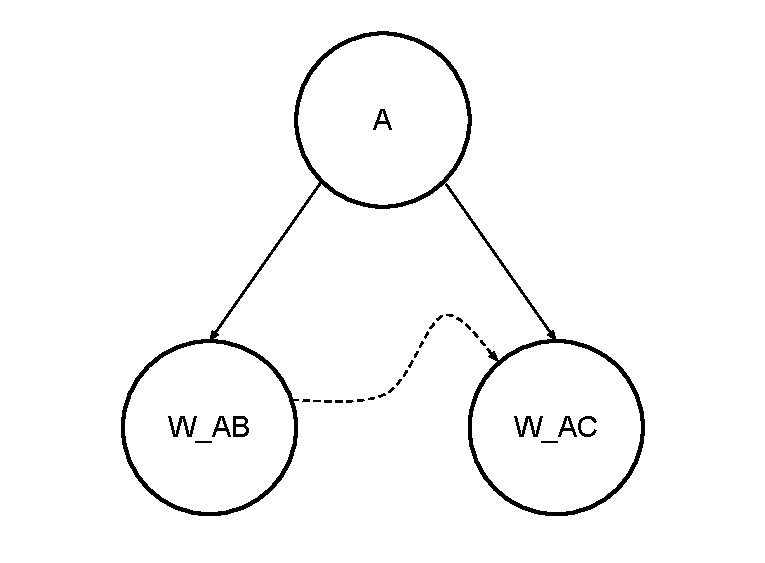
\includegraphics[width=\linewidth]
  {capitoli/figure/cap3/SchedulingConflictResolved.pdf}}$
  \subcaption{Dopo la risoluzione}
  \label{fig:schedulingConflictB}
 \end{minipage}
 \caption{Esempio di risoluzione di un conflitto tra due task.}
\label{fig:schedulingConflict}
\end{figure}

\paragraph{Definizione dell'ordine di scheduling}
Durante l'esecuzione dell'algoritmo di scheduling illustrato nella Sezione 
\ref{subsec:faseScheduling} si possono avere più task eleggibili per essere 
schedulati nello stesso passo, ovvero più task con le stesse precedenze 
soddisfatte. Si consideri la Figura \ref{fig:schedulingConflict} per un 
semplice esempio di conflitto tra due task. La Figura 
\ref{fig:schedulingConflictA} rappresenta una parte del task graph, 
nell'ipotesi che al passo corrente il task $A$, di colore grigio, sia già stato 
schedulato mentre i due task di comunicazione $W\_AB$ e $W\_AC$, di colore 
azzurro, sono eleggibili per il passo di scheduling successivo. Quando questa
situazione si verifica, l'algoritmo deve effettuare una decisione su quale 
task è meglio considerare per primo; tale scelta esplicita una relazione 
d'ordine tra i task in conflitto, rappresentata da un arco aggiuntivo inserito 
nella fase di postprocessing. La Figura \ref{fig:schedulingConflictB} 
rappresenta l'arco aggiuntivo inserito tra i due task di comunicazione, 
nell'ipotesi che il task $W\_AB$ sia stato scelto prima di $W\_AC$.

È importante evidenziare come i conflitti effettivi si abbiano solo tra task 
che sono eleggibili per lo scheduling in uno stesso passo e, soprattutto, che 
il componente su cui sono mappati sia lo stesso. Infatti, è sempre possibile 
che più task eleggibili durante lo stesso passo vengano poi eseguiti in 
parallelo, a prescindere dall'ordine con cui sono stati considerati 
dall'algoritmo; si ha un vero conflitto solo quando la loro esecuzione implica 
l'utilizzo di uno stesso componente. In tal caso, infatti, le esecuzioni devono 
necessariamente essere serializzate, per questo motivo tali task sono in 
conflitto.

\paragraph{Analisi dell'output dello scheduler}
I conflitti descritti nel precedente paragrafo sono ricavati dall'analisi 
dell'output dello scheduler durante la fase di postprocessing. Il diagramma di 
Gantt viene analizzato per ricavare le informazioni su tutti i task schedulati 
per ogni componente. A questo punto, partendo dalla lista dei task ordinata 
secondo l'ordine di esecuzione, al grafo vengono aggiunti degli archi che 
collegano i task nello stesso ordine in cui compaiono nella lista. In questo 
modo le informazioni sull'ordine scelto dallo scheduler vengono incluse nel 
task graph finale sotto forma di precedenze aggiuntive.

\paragraph{Scrittura dei dati su file XML}
Dopo aver analizzato il diagramma di Gantt e aver aggiunto gli archi seguendo 
l'ordine di scheduling, le informazioni rilevanti per il runtime manager 
vengono scritte nel file XML del progetto di \ac{FASTER}. I dati scritti sono:
\begin{itemize}
 \item tutte le implementazioni usate dai task che compongono il task graph 
finale, incluse implementazioni aggiuntive create ex novo per i task di 
comunicazione e di riconfigurazione;
 \item la lista dei mapping fornita dal mapper per i task di computazione, con 
mapping aggiuntivi per i task di comunicazione e riconfigurazione, che 
specificano l'implementazione da utilizzare e il componente su cui verranno 
eseguiti (componenti di comunicazione per i primi, controllore della 
riconfigurazione per i secondi);
 \item informazioni sul task graph finale, cioè con ordine di scheduling 
esplicito.
\end{itemize}

Tutte queste informazioni verranno poi utilizzate dal runtime manager per 
gestire l'effettiva esecuzione dell'applicazione.

Nella prossima sezione verrà descritta la parte più importante dell'algoritmo 
di scheduling, ossia la scelta di quale task è meglio considerare ad ogni 
passo.


\section{Euristica di scelta dei task}
\label{sec:euristicaSceltaTask}
In questa sezione viene spiegato come l'algoritmo di scheduling opera ad ogni 
passo la scelta di quale task è più conveniente considerare per l'assegnazione 
dei tempi, così da minimizzare la lunghezza totale dello schedule finale.

\paragraph{Utilizzo di un algoritmo euristico}
Come visto nel Capitolo \ref{chap:SOA}, è stato preferito l'utilizzo di un 
algoritmo euristico basato su una lista con uno scheduling effettuato 
iterativamente e in maniera incrementale, rispetto a una euristica 
esplorativa/evolvibile, che richiede un tempo di esecuzione superiore prima di 
giungere a risultati accettabili e rischia di generare molte soluzioni non 
applicabili. Allo stesso tempo, il procedimento di scegliere un task ad ogni 
passo sulla base di una determinata priorità, pur essendo molto veloce 
rappresenta una scelta \emph{greedy}, che può non garantire il 
raggiungimento di obiettivi accettabili.

Per questo è importante considerare diversi fattori e combinarli; sulla 
base di conoscenze pregresse è possibile identificare comportamenti 
ricorrenti che si verificano durante l'esecuzione di una generica applicazione, 
ad esempio possibili colli di bottiglia nell'esecuzione. Queste regolarità 
riscontrabili portano alla formulazione di diversi parametri che possono essere 
combinati nel calcolo della priorità che caratterizza ogni task, creando una 
funzione di priorità ``pesata'' rispetto alle possibili cifre di merito. Questo 
è l'approccio alla base dell'euristica utilizzata per la scelta dei task che 
viene illustrata in questa sezione.

\paragraph{Garanzia di applicabilità delle soluzioni generate}
L'algoritmo di scheduling proposto permette di evitare che vengano generate 
delle soluzioni \emph{infeasible}, soluzioni che violino i vincoli sul tempo di 
esecuzione (per esempio nel caso di tempi di esecuzione sovrapposti per task 
mappati sullo stesso componente), oppure che siano caratterizzate da un mancato 
rispetto delle precedenze tra i task del grafo.

Si assiste quindi alla generazione di una soluzione sempre valida per 
costruzione, poichè i task presi in esame ad ogni passo dall'euristica di 
scelta sono soltanto quelli le cui precedenze siano già state considerate. 
Questa caratteristica dell'algoritmo, combinata a una veloce euristica di scelta 
dei task, permette di ottenere in un tempo molto breve una soluzione che non 
viola nessun vincolo e che fornisce una stima del tempo di esecuzione fedele, 
nell'ipotesi che le stime dei tempi di esecuzione siano ragionevolmente 
affidabili.


\subsection{Funzionamento}
L'algoritmo per la scelta del task migliore viene invocato a ogni passo di 
scheduling, e opera su una lista aggiornata di task le cui precedenze sono 
soddisfatte.

Appena inizia l'esecuzione dell'algoritmo viene effettuata un'analisi 
preliminare della lista dei task per determinare se la lista contiene un solo 
elemento, ad esempio nel caso in cui si stia esaminando il primo nodo del 
grafo. Se si verifica questa situazione, allora l'unico elemento della lista è 
selezionato come task migliore. Nel caso in cui la lista contenga più di un 
elemento, è necessario procedere al calcolo delle priorità.

Viene eseguito un ciclo su tutta la lunghezza della lista, ad ogni passo del 
ciclo si calcola la priorità del task secondo il procedimento descritto nella 
prossima sezione; la priorità viene confrontata con la massima priorità trovata 
fino a quel momento. Dopo che tutti i task sono stati presi in esame, il task 
con la massima priorità in assoluto viene selezionato per l'assegnazione dei 
tempi, e l'algoritmo termina.


\subsection{Calcolo delle priorità}
Il calcolo della priorità di un task dipende dal suo tipo; diverse regole e 
modi per assegnare la priorità sono utilizzati a seconda che il task sia di 
computazione, comunicazione o riconfigurazione. Anche l'implementazione 
utilizzata per i task di computazione riveste un ruolo importante per definire 
come calcolare la priorità.

\subsubsection{Task con implementazione software}
I task con implementazione di tipo software non possono essere eseguiti su 
scheda, bensì vengono mappati su un processore general-purpose. Partendo da 
questo presupposto, la metrica utilizzata per calcolare la priorità di un task 
mappato con implementazione software è basata sulle informazioni sul percorso 
critico. In questo ambito diventano rilevanti tali informazioni, calcolate 
in precedenza durante la fase di preprocessing.

A seconda che il task sia o meno sul percorso critico del grafo, e in 
base all'eventuale scarto se così non è, viene calcolata la priorità del task 
di computazione. La funzione di calcolo della priorità dei task di computazione 
con implementazione software diventa quindi
\begin{equation} \label{eq:softwarePriority}
 f=C*CPInfo
\end{equation}
dove $C$ rappresenta un parametro costante e $CPInfo$ le informazioni sul 
percorso critico.

\subsubsection{Task con implementazione hardware}
Nel caso di task che devono essere eseguiti su logica riconfigurabile, quindi 
mappati su implementazioni di tipo hardware, vengono utilizzate tre metriche:
\begin{enumerate}
 \item informazioni sul percorso critico, come nel caso dei task con 
implementazione di tipo software;
 \item l'istante di inizio al più presto, o \emph{\ac{EST}}: rappresenta 
l'istante al più presto nel quale il task può iniziare l'esecuzione.
 \item l'istante di fine al più presto, o \emph{\ac{EFT}}.
\end{enumerate}
La funzione di calcolo della priorità risulta quindi diversa rispetto alla 
\ref{eq:softwarePriority}, assumendo la forma
\begin{equation} \label{eq:hardwarePriority}
 f=-A*EST - B*EFT + C*CPInfo
\end{equation}
dove $A$, $B$ e $C$ sono parametri fissati e $CPInfo$, $EST$ e $EFT$ sono le 
tre metriche sopra elencate.

Nei prossimi paragrafi viene descritto come si calcolano le tre metriche 
utilizzate nelle funzioni \ref{eq:softwarePriority} e \ref{eq:hardwarePriority}.

\paragraph{Informazioni sul percorso critico}
Il calcolo della metrica relativa al percorso critico si basa sulle 
informazioni riguardanti lo \emph{scarto} (slack) del task. I dati sugli 
scarti di tutti i task sono stati calcolati durante la fase di preprocessing, 
e sono disponibili in quanto inseriti nell'interfaccia di input dello scheduler.

Si fissa una soglia per lo scarto al di sotto della quale si considera il task 
come facente parte del percorso critico; al task si assegna quindi la massima 
priorità per questa cifra di merito se il suo scarto è sotto soglia. La 
definizione di una soglia permette all'algoritmo di essere meno rigido nel 
controllo dello scarto di un task, che viene così considerato come critico anche 
se il suo scarto è di poco superiore a $0$, invece che considerare critici 
solamente task con scarto nullo.

Se, invece, lo scarto del task supera la soglia, si considera il logaritmo di 
tale scarto. Il valore della cifra di merito è così calcolato:
\begin{equation}
 CPInfo = \begin{cases}
           MAX & \mbox{se } 0 \leq s \leq THRESHOLD\\
           \frac{1}{log_2\left(s\right)} & \mbox{se } s > THRESHOLD
          \end{cases}
\end{equation}
dove $s$ è lo scarto del task.

\paragraph{Earliest Start Time}
L'istante al più presto nel quale il task può iniziare l'esecuzione, senza 
contare possibili conflitti nell'utilizzo dei componenti, è concettualmente 
uguale al tempo \emph{asap}, anch'esso calcolato nella fase di preprocessing 
come lo scarto. Il valore della cifra di merito è così calcolato:
\begin{equation}
 EST = \begin{cases}
        0 & \mbox{se } asap = 0\\
        log_2\left(asap\right) & \mbox{se } asap > 0
       \end{cases}
\end{equation}
Si è deciso di utilizzare il logaritmo in modo da non penalizzare 
significativamente task che hanno un EST più elevato rispetto a task con un EST 
minore. Il logaritmo infatti permette di basarsi sulla differenza tra gli ordini 
di grandezza in base $2$.
% TODO spiegare cosa l'est permette di considerare

\paragraph{Earliest Finish Time}
L'istante al più presto in cui il task termina l'esecuzione è calcolato come la 
stima asap del task, a cui viene sommato il tempo di esecuzione stimato.

Il valore di questa metrica è così calcolato:
\begin{equation}
 EFT = log_2\left(asap + eTime\right)
\end{equation}
Si noti che il caso in cui l'argomento del logaritmo abbia valore $0$ non è 
gestito, poichè il tempo di esecuzione di un task di computazione è supposto 
non nullo, e l'unico caso in cui si abbia una stima $asap$ pari a $0$ si 
verifica nell'analisi dei task iniziali, che si suppone siano sempre task di 
computazione.

Valgono considerazioni analoghe rispetto alla precedente cifra di merito 
per quanto concerne l'uso del logaritmo nel calcolo del valore.
% TODO spiegare cosa l'eft permette di considerare

\subsection{Regole aggiuntive}
Oltre al calcolo delle varie metriche presentato nella precedente sezione, sono 
state introdotte delle regole aggiuntive che modificano i valori delle cifre di 
merito e, di conseguenza, della priorità finale dei task. Queste regole non 
operano avendo conoscenza isolata a livello del singolo task, bensì agiscono in 
base al comportamento tenuto in precedenza dall'algoritmo o considerando anche 
altri task. L'aggiunta di queste regole consente quindi all'algoritmo di 
effettuare scelte più ``intelligenti'' nella scelta dei task migliori da 
schedulare.

\subsubsection{Fattore di degrado}
La prima di queste tecniche è l'introduzione di un \emph{fattore di degrado} 
(in inglese \emph{decay factor}). Può capitare che, nel corso dell'esecuzione 
dello scheduler, venga data sempre massima priorità ai task sul percorso 
critico, che vengono quindi scelti dall'euristica come migliori a ogni passo di 
scheduling. Laddove vi siano molti conflitti (soprattutto nelle comunicazioni) 
questo può portare al verificarsi di un collo di bottiglia nell'utilizzo delle 
risorse, che vengono occupate prevalentemente da task che si trovano sul 
percorso critico, mentre altri task non possono essere eseguiti per la continua 
occupazione delle risorse su cui questi sono mappati.

Per scongiurare il verificarsi di questa situazione, si è deciso di introdurre 
un fattore di degrado, che riduca progressivamente il massimo valore della 
cifra di merito corrispondente alle informazioni sul percorso critico; in 
questo modo viene data una sempre minore priorità ai task sul percorso critico. 
Il fattore di degrado è inizialmente unitario, così da avere impatto nullo; man 
mano che si scelgono task sul percorso critico esso viene ridotto 
progressivamente di una quantità $\delta_1$. Non appena viene scelto un 
task che non appartiene al percorso critico (quindi avente scarto sopra la 
soglia), il fattore di degrado viene incrementato di una quantità $\delta_2$. 
In questo modo, se non si scelgono task sul percorso critico si torna a dare 
maggiore priorità ai task critici.

L'assegnamento del valore alla cifra di merito relativa al task critico, 
delineato nella \ref{eq:softwarePriority}, viene sostituito con
\begin{equation} \label{eq:newSoftwarePriority}
 CPInfo = \begin{cases}
           MAX*df & \mbox{se } 0 \leq s \leq THRESHOLD\\
           \frac{1}{log_2\left(s\right)} & \mbox{se } s > THRESHOLD
           \end{cases}
\end{equation}
dove $df$ rappresenta il fattore di degrado.

\subsubsection{Priorità per task di comunicazione}
La seconda tecnica utilizzata è una diversa assegnazione di priorità per alcuni 
task di comunicazione. Come visto nella Sezione 
\ref{sec:aggiuntaRiconfigurazioni}, eventuali task di riconfigurazione vengono 
inseriti tra i task di comunicazione di tipo \emph{WRITE} e \emph{READ} che 
leggono e scrivono dati su quell'area, rispettivamente. Poichè il tempo 
impiegato per la riconfigurazione di un'area in generale introduce un 
overhead considerevole nell'esecuzione dell'applicazione, è auspicabile che 
il tempo di riconfigurazione venga ``nascosto'' il più possibile dal tempo 
impiegato per l'esecuzione di altri task (le dipendenze del task da eseguire 
successivamente sull'area riconfigurata), così da non introdurre ritardi che 
peseranno sul makespan finale.

Per mascherare il più possibile l'esecuzione di una riconfigurazione è 
necessario che questa parta il prima possibile, il che implica, per la 
struttura del grafo costruito dopo la fase di preprocessing, che tutte le 
comunicazioni di tipo \emph{WRITE} che precedono la riconfigurazione vengano 
eseguite il prima possibile. Questo requisito è stato risolto creando una 
regola speciale per il calcolo della priorità dei task di comunicazione di tipo 
\emph{WRITE} che precedono una riconfigurazione; per questi tipi di task, la 
priorità è calcolata nel seguente modo:
\begin{equation} \label{eq:writeBeforeRecPriority}
 f=-A*EST - B*EFT + C*CPInfo + EP
\end{equation}
dove il termine aggiuntivo $EP$ rappresenta la priorità extra che viene 
assegnata ai task. La formula \ref{eq:writeBeforeRecPriority} sostituisce la 
\ref{eq:hardwarePriority} in questi casi.


\section{Elementi di comunicazione e gestione della memoria}
\label{sec:elementiComunicazioneGestioneMemoria}



\section{Osservazioni conclusive}
\label{sec:osservazioniConclusive}
In questa sezione viene fornito un riepilogo dei concetti importanti relativi 
alla metodologia proposta per risolvere il problema dello scheduling dei task 
per l'esecuzione di un applicazione su hardware riconfigurabile, considerando 
le comunicazioni e le riconfigurazioni.

\begin{itemize}
  \item Sono state definite delle interfacce di input e di output per 
l'algoritmo proposto, per consentire allo scheduler di avere conoscenza dei 
dati contenuti nel file XML di \ac{FASTER}, di rielaborarli e modificarli 
consentendo l'introduzione dei task di comunicazione e riconfigurazione, oltre 
al calcolo di informazioni rilevanti per l'esecuzione dell'euristica;
 \item L'obiettivo è fornire un algoritmo di scheduling che sia veloce, per 
consentire alla fase di esplorazione delle soluzioni di terminare in un tempo 
ragionevolmente breve. Questa necessità ha portato allo sviluppo di un algoritmo 
che non è basato su euristiche esplorative o evolvibili, ma sulla base di una 
lista di priorità e una scelta ``greedy'';
 \item Sono state introdotte delle regole aggiuntive, oltre al semplice calcolo 
delle metriche per assegnare le priorità ai task, che tengono conto di 
possibili colli di bottiglia che possono verificarsi durante l'esecuzione e 
cercano di ridurre l'impatto di tali fenomeni sulla lunghezza dello schedule.
% TODO qualche altra cosa che può venire in mente
\end{itemize}
